\documentclass{beamer}

\usepackage[french]{babel}
\usepackage[T1]{fontenc}
\usepackage[export]{adjustbox}
\usepackage{graphicx}
\usepackage{blkarray} % Required for inserting images
\usepackage{svg}

\newcommand{\nologo}{\setbeamertemplate{logo}{}}

\mode<presentation>{
  \useinnertheme{rectangles}
  \usecolortheme[rgb={0.3,0.5,0.8}]{structure}
  \usecolortheme{orchid}
  \usecolortheme{whale}
  \useoutertheme{infolines}
  \setbeamercovered{transparent}
}

\graphicspath{ {./images/} }

\title{Jeu de plate-formes avec génération procédurale}
\subtitle{Projet semestriel}
\author[T.Pariney L.Jaqueson K.Jelic]{Théo Pariney \newline Laura Jacqueson \newline Kilian Jelic\\\footnotesize Tuteur : Julien Bernard}
\institute[]{Université Marie et Louis Pasteur \\ \vspace{0.25cm} Licence 3 Informatique, 2024--2025}
\date{26 mars 2025}
\logo{
\includegraphics[width=0.25\linewidth]{images/logo-UMLP}}

\AtBeginSection[]
{
  \begin{frame}<beamer>
    \frametitle{Plan}
    \tableofcontents[currentsection,currentsubsection,subsubsectionstyle=show/show/hide/hide]
  \end{frame}
}

\begin{document}

\begin{frame}
    \titlepage
\end{frame}

{\nologo

\begin{frame}{Plan}
    \tableofcontents
\end{frame}

\begin{frame}{Introduction}
    \begin{block}{Qu'est-ce qu'un jeu de plateforme ?}
       \begin{itemize}
            \item[\bullet] Personnage qui saute sur des plateformes
            \item[\bullet] Défilement horizontal ou vertical
            \item[\bullet] Collecte d'objets
            \item[\bullet] Obstacles
        \end{itemize}
    \end{block}
    \begin{block}{Contexte et objectifs}
        \begin{itemize}
            \item[\bullet] Jeu de plateformes en 2D
            \item[\bullet] Réalisé en C++
            \item[\bullet] Génération procédurale
            \item[\bullet] Utilise la bibliothèque : Gamedev Framework
        \end{itemize}
    \end{block}
\end{frame}

\section{Présentation du jeu}
\begin{frame}{Présentation du jeu}
    \begin{block}{Caract\'eristiques}
        \begin{itemize}
            \item[\bullet] Jeu de plateforme en 2D en C++
            \item[\bullet] Personnage : petit robot
            \item[\bullet] Contrôles
            \begin{itemize}
                \item droite et gauche
                \item saut et double saut
                \item dash : impulsion rapide horizontal
            \end{itemize}
            \item[\bullet] Niveau : pas de choix $\rightarrow$ génération aléatoire
            \item[\bullet] Missions du personnage : ramasser écrous et rejoindre sortie
        \end{itemize}
    \end{block}
\end{frame}

\begin{frame}{Objectifs du jeu}
    \begin{columns}
        \column{0.5\textwidth}
        \begin{block}{Score : objets ramassables}
            \begin{itemize}
                \item[\bullet] Types : écrous
                \item[\bullet] Nombre inconnu
                \item[\bullet] Tous placés aléatoirement
                \item[\bullet] Pas d'obligation de collecte
            \end{itemize}
        \end{block}
        \begin{block}{Sortie}
            \begin{itemize}
                \item[\bullet] Placée aléatoirement
                \item[\bullet] Stop la partie
            \end{itemize}
        \end{block}
        \column{0.4\textwidth}
        \begin{figure}
            \centering
            
\includegraphics[width=0.6\textwidth]{nut}
        \end{figure}
        \begin{figure}
            \centering
            
\includegraphics[width=0.6\textwidth]{exit}
        \end{figure}

    \end{columns}
\end{frame}

\section{Blocs et textures}
\begin{frame}{Stockage dynamique des blocs}
    \begin{columns}
        \column{0.6\textwidth}
            \begin{figure}
                \centering
                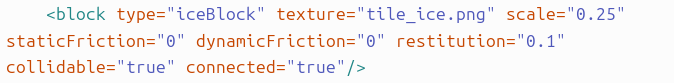
\includegraphics[width=1.0\textwidth]{XMLfile}
            \end{figure}
        \column{0.4\textwidth}
            \begin{block}{Définition des blocs}
                \begin{itemize}
                    \item[\bullet] Définition des blocs au format XML
                    \item[\bullet] Lecture du fichier et stockage dans une classe dédiée
                    \item[\bullet] Accès depuis les autre classes via une méthode statique
                \end{itemize}
            \end{block}
    \end{columns}
\end{frame}

\begin{frame}{Contenu  du fichier XML}
    \begin{block}{Attributs des blocks}
        \begin{itemize}
            \item[\bullet] Type principal
            \item[\bullet] \textbf{type} : Sous-type du bloc
            \item[\bullet] \textbf{texture} : Texture du bloc
            \item[\bullet] \textbf{scale} : Échelle de la texture
            \item[\bullet] \textbf{staticFriction/dynamicFriction} : Coefficients de friction
            \item[\bullet] \textbf{restitution} : Coefficients de réstitution
            \item[\bullet] \textbf{collidable} : Collision possible
            \item[\bullet] \textbf{connected} : Textures connectées
            \item[\bullet] \textbf{direction} : Direction des platformes connectées
            \item[\bullet] \textbf{alternate} : Texture alternative
        \end{itemize}
    \end{block}
\end{frame}

\begin{frame}{Connectivité des textures}
    \begin{columns}
        \column{0.4\textwidth}
            \begin{block}{Textures connectées}
                \begin{itemize}
                    \item[\bullet] Textures différentes en fonction des blocs autour
                    \item[\bullet] élément \emph{connected} du fichier XML
                    \item[\bullet] Connectivité entre les groupes de blocs
                    \item[\bullet] Format de feuille de sprites
                \end{itemize}
            \end{block}
        \column{0.6\textwidth}
            \begin{figure}
                \centering
                
\includegraphics[width=0.4\textwidth]{images/connectedTiles.png}
            \end{figure}
            \begin{figure}
                \centering
                
\includegraphics[width=1.0\textwidth]{images/tile_jelly.png}
            \end{figure}
    \end{columns}
\end{frame}

\begin{frame}{Calcul des textures}
    \begin{columns}
        \column{0.4\textwidth}
            \begin{block}{Textures connectées}
                \begin{itemize}
                    \item[\bullet] Bit donné à chaque bloc autour
                    \item[\bullet] Somme des bits donne la texture dans la feuille de sprites
                \end{itemize}
            \end{block}
        \column{0.6\textwidth}
            \begin{figure}
                \centering
                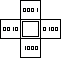
\includegraphics[width=0.8\textwidth]{images/connected_textures_offset_computing.png}
            \end{figure}
    \end{columns}
\end{frame}

\section{Présentation du personnage}
\begin{frame}{Contrôles de base}
    \begin{columns}
        \column{0.6\textwidth}
            \begin{block}{Contrôles du personnage}
                \begin{itemize}
                    \item[\bullet] Direction droite et gauche
                    \item[\bullet] Touches \emph{D} et \emph{Q}
                    \item[\bullet] Touches $\rightarrow$ et $\leftarrow$
                    \item[\bullet] Priorité à la direction droite
                \end{itemize}
            \end{block}
        \column{0.4\textwidth}
            \begin{figure}
                \centering
                
\includegraphics[width=0.8\textwidth]{character_placeholder}
            \end{figure}
    \end{columns}
\end{frame}

\begin{frame}{Saut}
    \begin{block}{Saut}
        \begin{itemize}
            \item[\bullet] Touche \emph{Espace}
            \item[\bullet] Impulsion vers le haut instantanée
            \item[\bullet] Redescente sous l'effet de la gravité 
            \item[\bullet] Permet de franchir des obstacles
        \end{itemize}
    \end{block}
\end{frame}

\begin{frame}{Saut}
    
    \begin{block}{Double saut}
        \begin{itemize}
            \item[\bullet] Touche \emph{Espace} en l'air
            \item[\bullet] Utilisable une fois par saut
            \item[\bullet] Réinitialisation en touchant le sol
            \item[\bullet] Permet l'accès à des plateformes très haute
        \end{itemize}
    \end{block}
    \begin{figure}
        \centering
        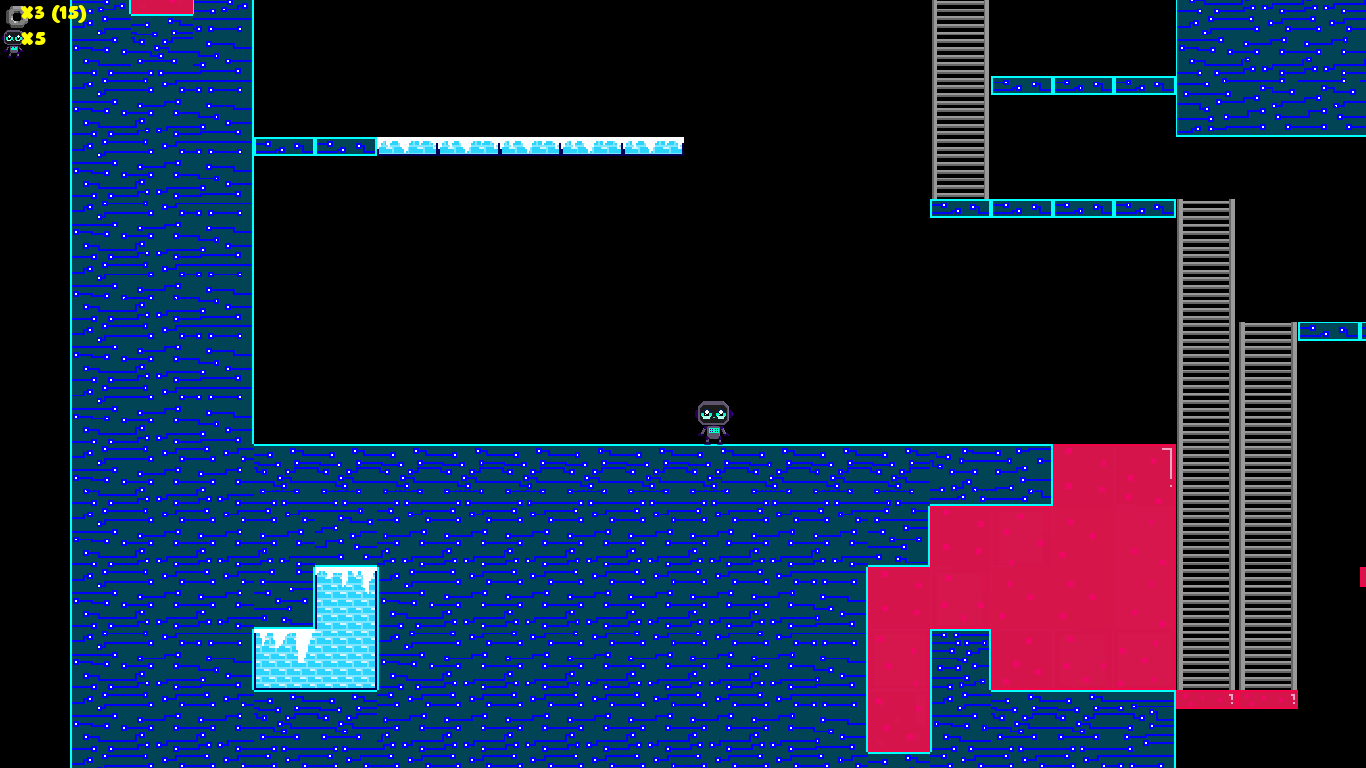
\includegraphics[width=0.55\textwidth]{images/double_jump_ex.png}
    \end{figure}
\end{frame}

\begin{frame}{Dash}
    \begin{block}{Dash}
        \begin{itemize}
            \item[\bullet] Impulsion directionnelle instantanée
            \item[\bullet] Double appui : D, Q ou $\rightarrow$, $\leftarrow$
            \item[\bullet] Temps de recharge
            \item[\bullet] Permet de passer un grand espace vide
            
        \end{itemize}
    \end{block}
    \begin{figure}
        \centering
        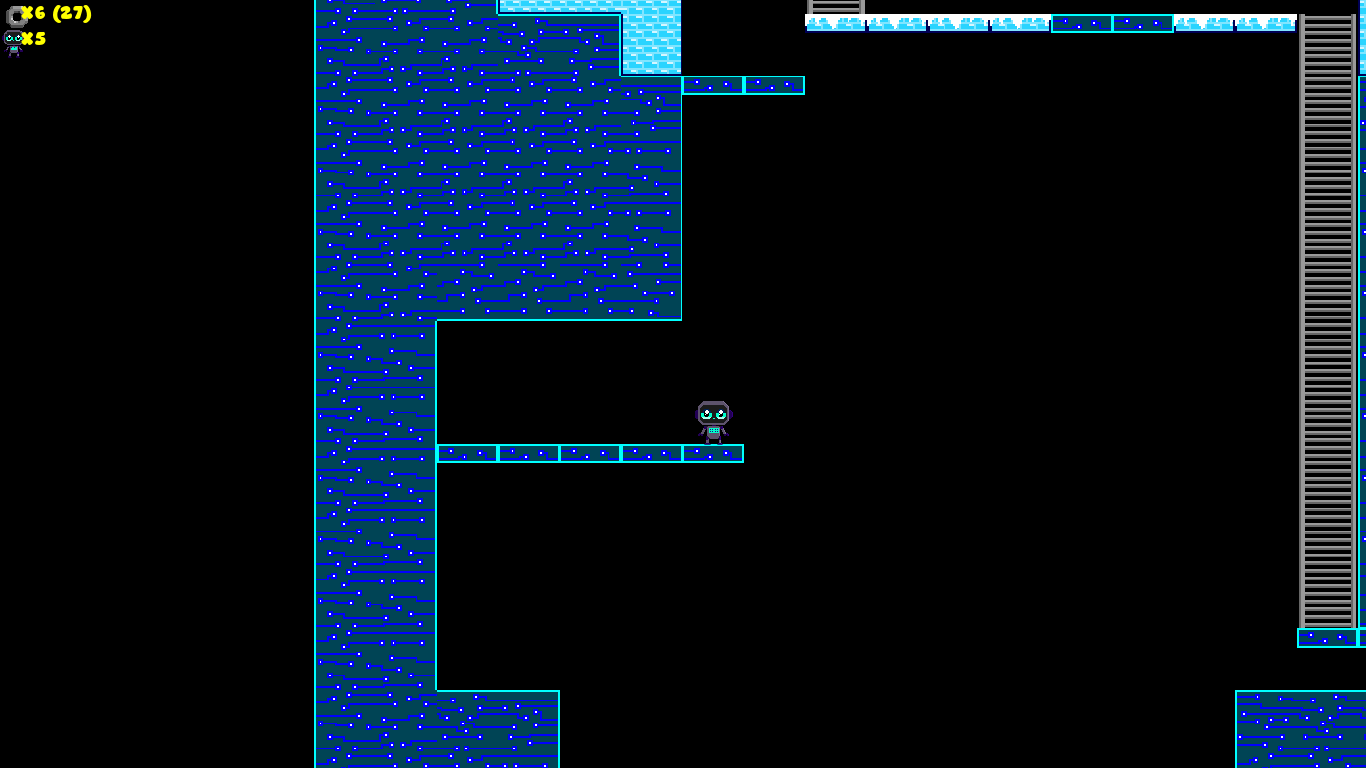
\includegraphics[width=0.55\textwidth]{images/dash_ex.png}
    \end{figure}
\end{frame}

\begin{frame}{Score et vies}
    \begin{columns}
        \column{0.6\textwidth}
            \begin{block}{Vies du personnage}
                \begin{itemize}
                    \item[\bullet] Diminution au contact d'un pique : mort
                    \item[\bullet] 5 vies au total
                    \item[\bullet] Fin de la partie à 0
                \end{itemize}
            \end{block}
            \begin{block}{Score}
                \begin{itemize}
                    \item[\bullet] Incrémentation en touchant un écrou
                \end{itemize}
            \end{block}
        \column{0.4\textwidth}
            \begin{figure}
                \centering
                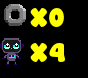
\includegraphics[width=0.8\textwidth]{Screenshot from 2025-03-23 23-14-37}
            \end{figure}
    \end{columns}
\end{frame}

\section{Génération procédurale}
\begin{frame}{L'al\'eatoire}
    \begin{block}{Graine de génération}
        \begin{itemize}
            \item[\bullet] Choix aléatoire
            \item[\bullet] Choix manuel
            \item[\bullet] Reproduction des problèmes
        \end{itemize}
    \end{block}
\end{frame}

\begin{frame}{Génération des salles/des murs}
    \begin{columns}
        \column{0.5\textwidth}
        \begin{block}{Génération des salles}
            \begin{itemize}
                \item[\bullet] Génération d'une une suite de salles connectées entre elles
                \item[\bullet] Placement le long de la salle précédente
                \item[\bullet] Salles ne se chevauchant pas
                \item[\bullet] Retour en arrière si aucun chemin n'est possible
            \end{itemize}
        \end{block}
        \column{0.4\textwidth}
        \begin{figure}
            \centering
            
\includegraphics[width=0.9\textwidth]{room_placement}
        \end{figure}
        \begin{figure}
            \centering
            
\includegraphics[width=0.9\textwidth]{filling_the_world}
        \end{figure}
    \end{columns}
\end{frame}

\begin{frame}{Génération du chemin}
    \begin{columns}
        \column{0.5\textwidth}
        \begin{block}{Génération d'un chemin}
            \begin{itemize}
                \item[\bullet] Génération d'un chemin du début à la fin
                \item[\bullet] Niveau toujours possible
                \item[\bullet] Calcul dans deux directions
                \item[\bullet] Choix parmi les directions possibles
            \end{itemize}
        \end{block}
        \begin{block}{Changement de direction}
            \begin{itemize}
                \item[\bullet] Bloc solide
                \item[\bullet] Plafond atteint
            \end{itemize}
        \end{block}
        \column{0.4\textwidth}
        \begin{figure}
            \centering
            
\includegraphics[width=1.0\textwidth]{two_ways_to_connect}
        \end{figure}
    \end{columns}
\end{frame}

\begin{frame}{Les fausses plateformes}
    \begin{columns}
        \column{0.5\textwidth}
        \begin{block}{Pourquoi?}
            \begin{itemize}
                \item[\bullet] Vrai chemin caché
                \item[\bullet] Exploration du niveau
                \item[\bullet] Placement des écrous
            \end{itemize}
        \end{block}
        \column{0.4\textwidth}
        \begin{figure}
            \centering
            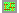
\includegraphics[width=1.0\textwidth]{fake_platforms}
        \end{figure}
    \end{columns}
\end{frame}

\begin{frame}{Les blocs spéciaux}
    \begin{columns}
        \column{0.5\textwidth}
        \begin{block}{Blocs de glace et de slime}
            \begin{itemize}
                \item[\bullet] Variété dans les déplacements
                \item[\bullet] Génération à partir d'un bruit de Perlin
            \end{itemize}
        \end{block}
        \begin{block}{Bruit de Perlin}
            \begin{itemize}
                \item[\bullet] Nombres aléatoires
                \item[\bullet] Positions proches \eq valeurs proches
                \item[\bullet] Allure de ``collines''
            \end{itemize}
        \end{block}
        \column{0.4\textwidth}
        \begin{figure}
            \centering
            
\includegraphics[width=0.4\textwidth]{perlin_noise_example}
        \end{figure}
        \begin{figure}
            \centering
            
\includegraphics[width=1.0\textwidth]{perlin_noise_gradient}
        \end{figure}
        \begin{figure}
            \centering
            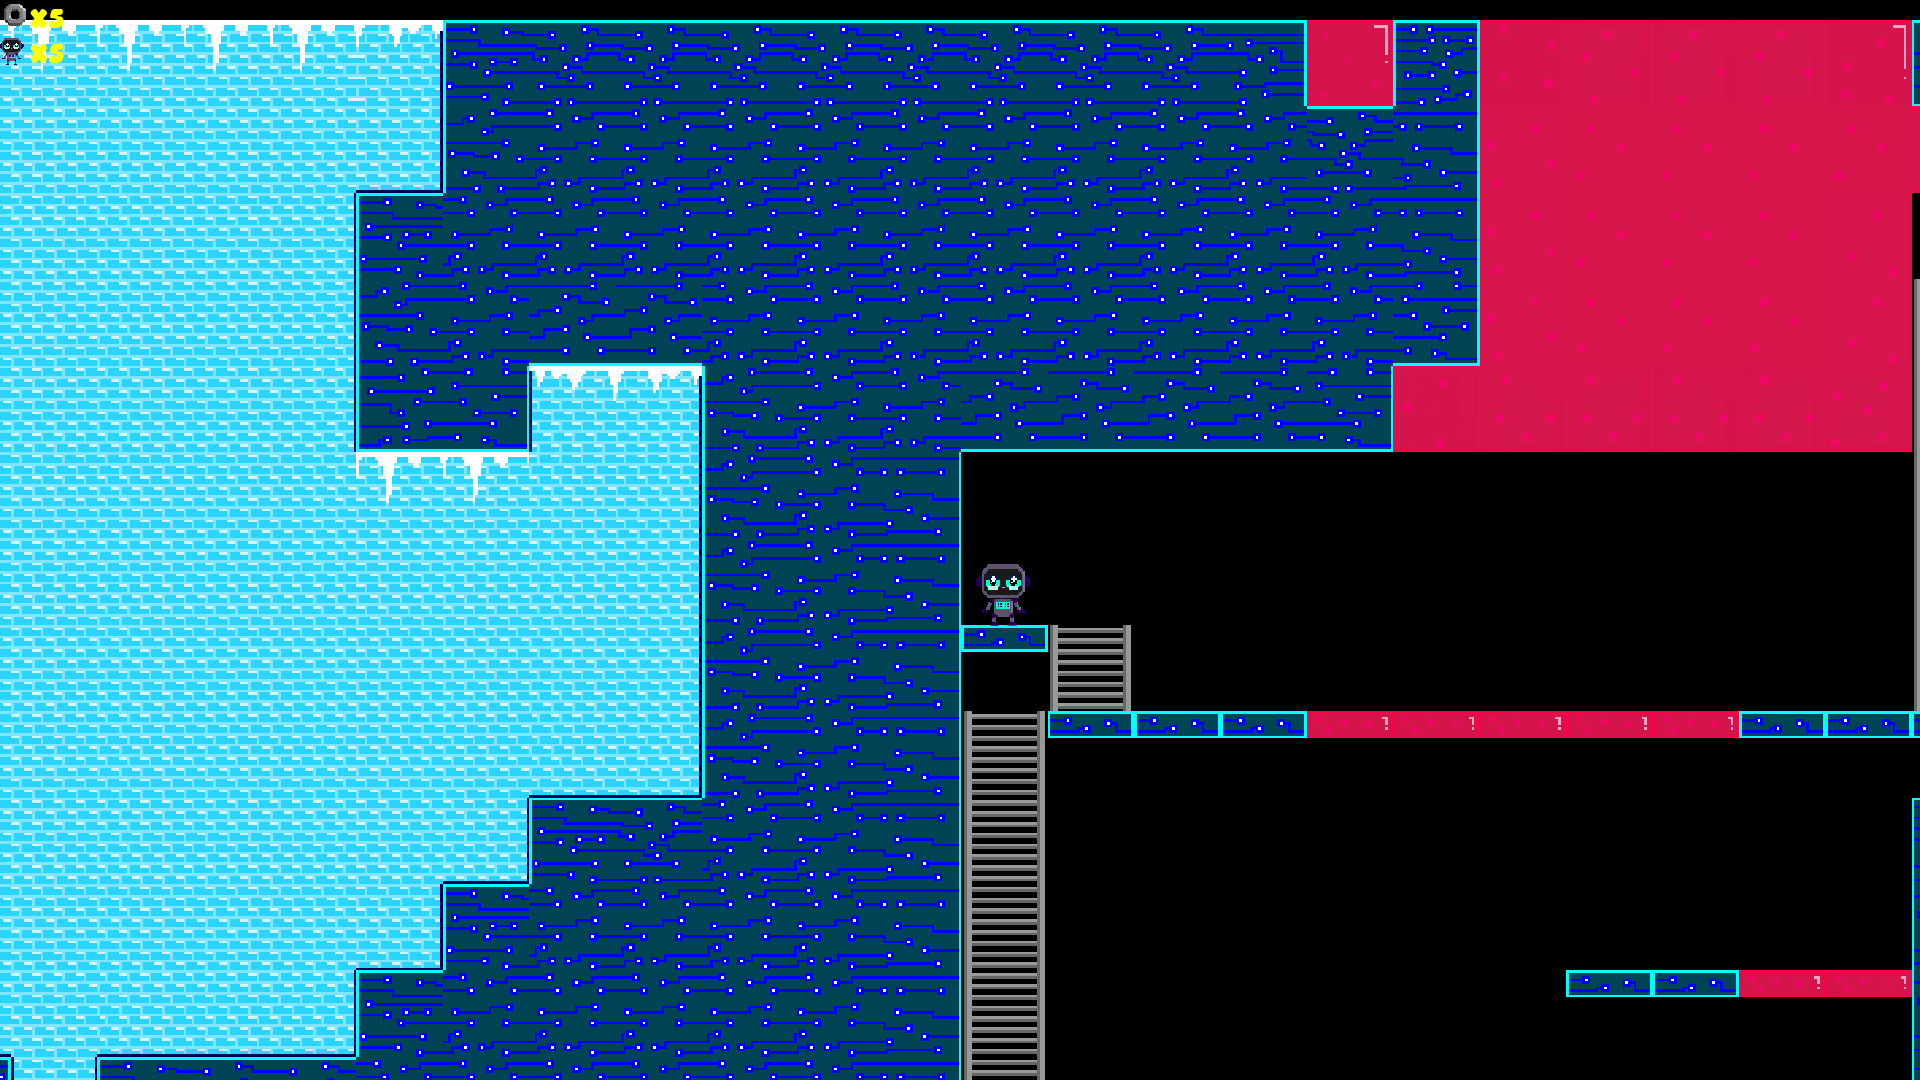
\includegraphics[width=1.0\textwidth]{perlin_noise_in_level}
        \end{figure}
    \end{columns}
\end{frame}

\begin{frame}{Les pièges}
    \begin{columns}
        \column{0.5\textwidth}
        \begin{block}{Génération de pics}
            \begin{itemize}
                \item[\bullet] 30\% de salles dangereuses
                \item[\bullet] Placement au sol des salles dangereuses
                \item[\bullet] Extrémités de lignes de blocs de glace
            \end{itemize}
        \end{block}
    \column{0.4\textwidth}
        \begin{figure}
            \centering
            
\includegraphics[width=1.0\textwidth]{ice_spike_trap}
        \end{figure}
    \end{columns}
\end{frame}

\begin{frame}{Point d'apparition}
    \begin{columns}
        \column{0.5\textwidth}
        \begin{block}{Point d'apparition du joueur}
            \begin{itemize}
                \item[\bullet] Début du niveau
                \item[\bullet] Endroit sûr
            \end{itemize}
        \end{block}
        \column{0.4\textwidth}
        \begin{figure}
            \centering
            
\includegraphics[width=1.0\textwidth]{valid_spawn_locations}
        \end{figure}
    \end{columns}
\end{frame}

\begin{frame}{Monde de test}
    \begin{block}{Monde de test}
        \begin{itemize}
            \item[\bullet] Monde alternatif
            \item[\bullet] Permet de tester les fonctionnalités
        \end{itemize}
    \end{block}
    \begin{figure}
        \centering
        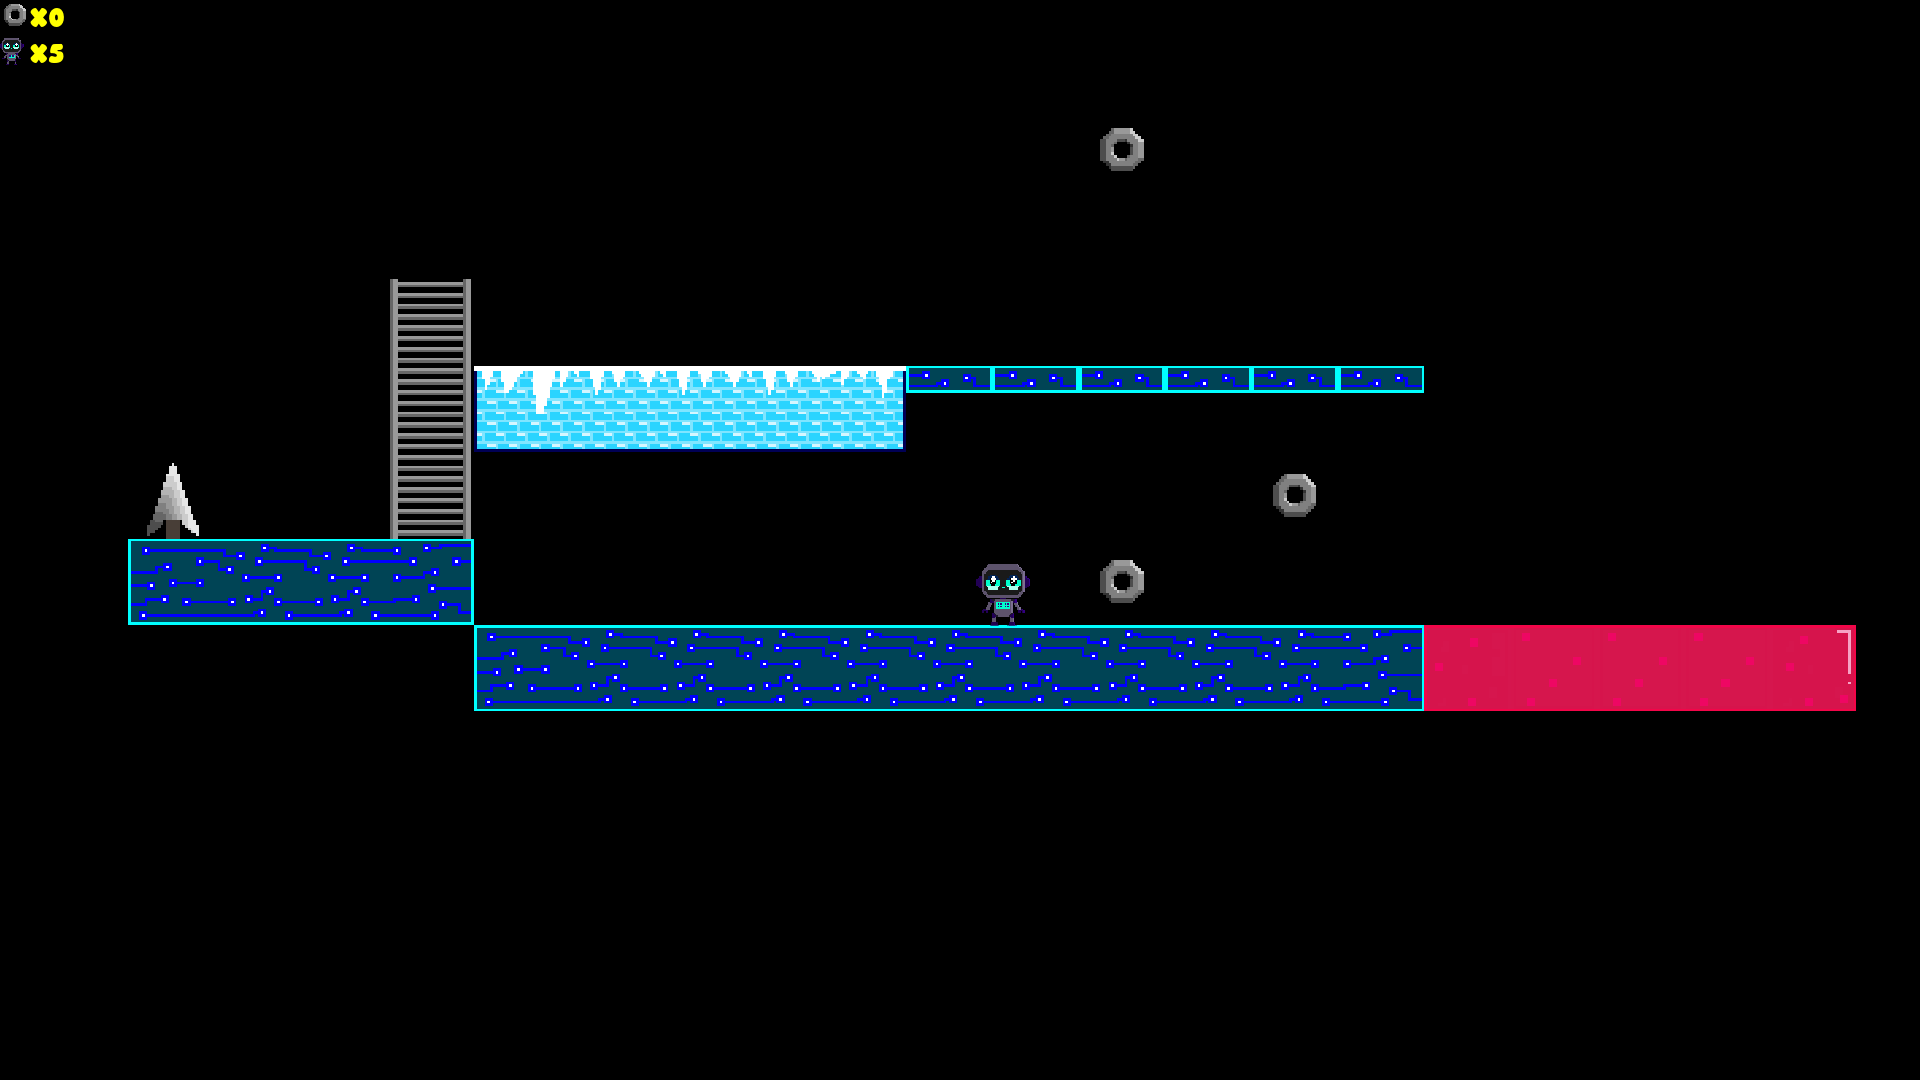
\includegraphics[width=0.7\textwidth]{test_world}
    \end{figure}
\end{frame}

\section{Physique}
\begin{frame}{Gestion des collisions}
    \begin{columns}
        \column{0.5\textwidth}
        \begin{block}{Collisions}
            \begin{itemize}
                \item[\bullet] Séparation de deux objets qui se rentrent dedans
                \item[\bullet] Collisions entre rectangles
                \item[\bullet] Collisions entre joueur et blocs seulement
            \end{itemize}
        \end{block}
        \begin{block}{Résolution des Collisions}
            \begin{itemize}
                \item[\bullet] Dépends du coefficient de restitution
                \item[\bullet] Nécessite d'appliquer une correction de position
            \end{itemize}
        \end{block}
        \column{0.4\textwidth}
        \begin{figure}
            \centering
            \includegraphics[width=1.0\textwidth]{images/schéma collision.png}
        \end{figure}
    \end{columns}
\end{frame}

\begin{frame}{Platformes directionnelles}
    \begin{columns}
        \column{0.5\textwidth}
            \begin{block}{Platformes directionnelles}
                \begin{itemize}
                    \item[\bullet] élément \emph{direction} du fichier XML
                    \item[\bullet] Joueur utilise une boîte de collisions plus petite
                \end{itemize}
            \end{block}
            \begin{block}{Détection de la collision}
                Collision résolue uniquement si :
                \[angle(Dir_{block},n) + \pi \le 10\%\]
            \end{block}
        \column{0.5\textwidth}
            \begin{figure}
                \centering
                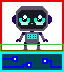
\includegraphics[width=0.5\textwidth]{DirectionnalHB}
            \end{figure}
    \end{columns}
\end{frame}

\begin{frame}{Friction}
    \begin{columns}
        \column{0.5\textwidth}
        \begin{block}{Résolution de la friction}
            \begin{itemize}
                \item[\bullet] Ralentis le joueur quand il se déplace sur un blocs
                \item[\bullet] Dépends des coefficients de friction dynamique et statiques des blocs
                \item[\bullet] Résolu après application de la résolution de collision
            \end{itemize}
        \end{block}
        \column{0.4\textwidth}
        \begin{figure}
            \centering
            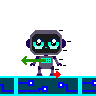
\includegraphics[width=1.0\textwidth]{images/Friction.png}
        \end{figure}
    \end{columns}
\end{frame}

\begin{frame}{Autre données de physique}
    \begin{block}{Résistance de l'air}
        L'air ralentis la vitesse du joueur
        \begin{figure}
            \centering
            
\includegraphics[width=0.2\textwidth]{images/Airresistance.png}
        \end{figure}
    \end{block}

    \begin{block}{Collisions multiples}
        Moyenne des résultats des collisions avec les blocs
    \end{block}
\end{frame}

\begin{frame}{Outils utilisés}
    \begin{block}{Outils pour le projet}
        \begin{itemize}
            \item[\bullet] Gamedev Framework (GF)
            \item[\bullet] Discord
            \item[\bullet] Google Docs
            \item[\bullet] Trello
            \item[\bullet] Git et Github
            \item[\bullet] IDEs (Kate, VScode, CLion)
        \end{itemize}
    \end{block}
\end{frame}

\section{Notre organisation}
\begin{frame}{Organisation du travail}
    \begin{block}{Notre organisation}
        \begin{itemize}
            \item[\bullet] Rendez-vous fréquent avec notre responsable
            \item[\bullet] Objectifs entre chaque rendez-vous
            \item[\bullet] Division de l'objectif en \emph{cartes} rangées par thème dans des \emph{listes} sur Trello
            \item[\bullet] Choix libre des tâches à faire pour chaque membre
        \end{itemize}
    \end{block}
\end{frame}

\section{Conclusion}
\begin{frame}{Conclusion}
    \begin{block}{R\'esultats}
        \begin{itemize}
            \item[\bullet] Projet réalisé dans son intégralité
            \item[\bullet] Objectifs fixés accomplis :
            \begin{itemize}
                \item[\rightarrow] Moteur physique cohérent
                \item[\rightarrow] Génération procédurale fonctionnelle
                \item[\rightarrow] Mécaniques du personnage variées
            \end{itemize}   
        \end{itemize}
    \end{block}
    \begin{figure}
        \centering
        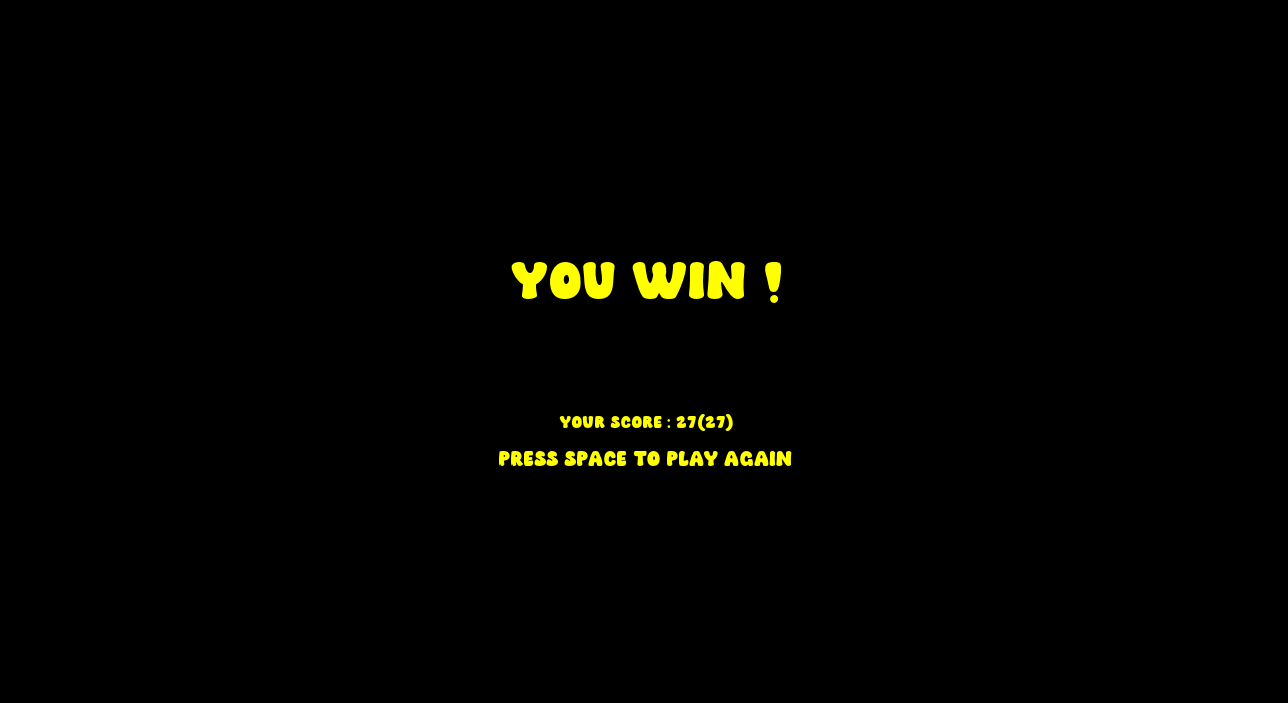
\includegraphics[width=0.58\textwidth]{images/end.png}
    \end{figure}
\end{frame}

\begin{frame}{Ce qu'on aurait voulu ajouter}
    \begin{block}{Elements d'amélioration}
        \begin{itemize}
          \item[\bullet] Des ennemis
          \item[\bullet] Possibilité de choix de la graine de génération
          \item[\bullet] Téléporteurs
          \item[\bullet] Des bonus
          \item[\bullet] Autre personnages
        \end{itemize}
    \end{block}
\end{frame}

\begin{frame}{Wave function collapse}
    \begin{columns}
        \column{0.5\textwidth}
        \begin{block}{Algorithme Wave Function Collapse}
            \begin{itemize}
                \item[\bullet] Arrange un ensemble de patternes donnés
                \item[\bullet] Pourrait être utilisé avec des morceaux de niveau
            \end{itemize}
        \end{block}
        \column{0.4\textwidth}
        \begin{figure}
            \centering
            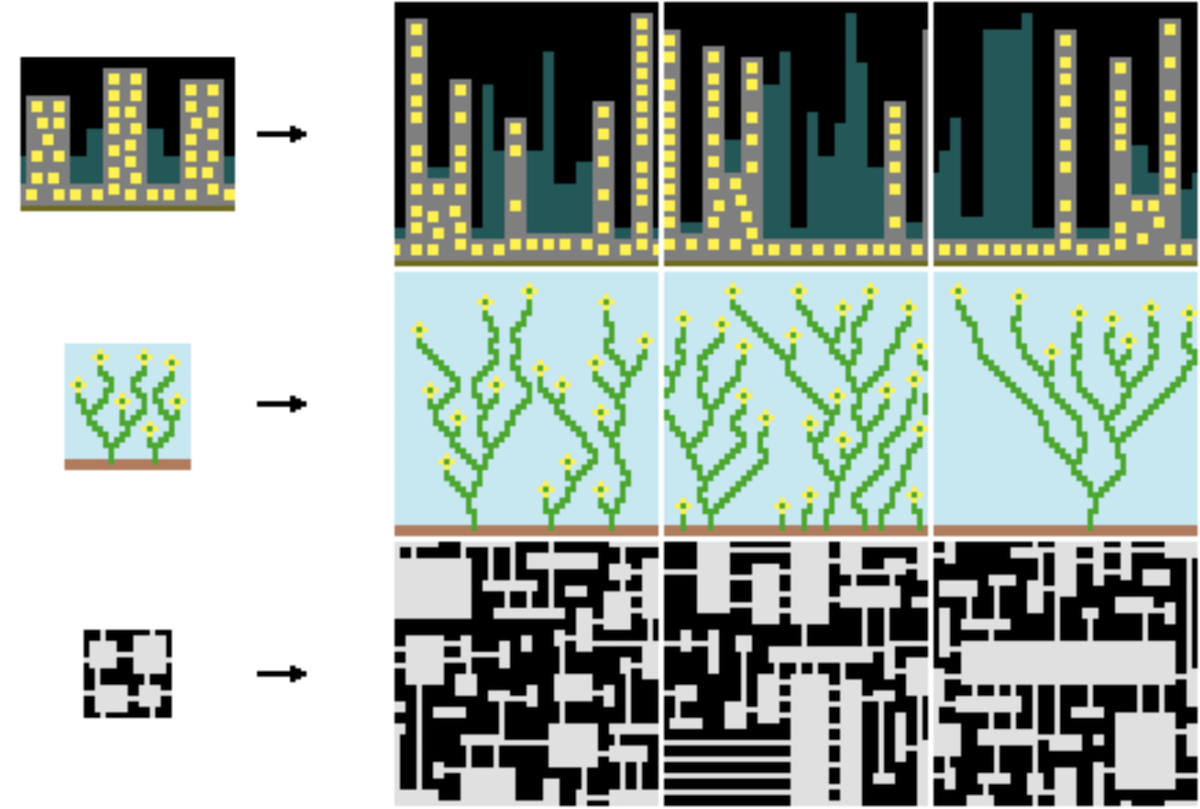
\includegraphics[width=1.0\textwidth]{wfc-examples}
            \caption{Des exemples d'application du Wave Function Collapse}
        \end{figure}
    \end{columns}
\end{frame}

}

\begin{frame}
    \centering
    Avez vous des questions ?
    \begin{figure}
        \centering
        
\includegraphics[width=0.5\linewidth]{character_placeholder}
    \end{figure}
\end{frame}

\end{document}
